\parindent=0em
\subsection{Aplicación}
\noindent

Debido al extenso número de factores a considerar a la hora de realizar las pruebas, implementamos una aplicación para automatizar las mismas y extraer los datos de ella. Estos datos se extraen mediante capturas de pantalla que se pueden realizar dentro de la aplicación. \\ 

El resultado obtenido no se limita a una única ejecución de la prueba, ya que esto produciría un sesgo en los mismos. Por ello cada prueba es realizada desde distintas perspectivas para tener otros factores en cuenta. Los factores determinantes pueden ser, por ejemplo, la luz natural del entorno o los objetos que en este se encuentren.\\ 

La forma ideal de realización de las pruebas seria mediante la iteración de estas sobre un archivo de vídeo previamente grabado. Sin embargo, ARCore no utiliza únicamente los datos extraídos de la entrada de vídeo. Tiene en cuenta a la hora de determinar la profundidad sensores del dispositivo como pueden ser el giróscopo o el acelerómetro, para medir rotaciones y posiciones, respectivamente.\\

La aplicación cuenta con un \textit{Asset} para facilitar la medición de los datos llamado Graphy. Este proporciona la medición de los Frames por segundo (FPS),uso de memoria y consumo de CPU de la aplicación así como todas las características internas del dispositivo. (https://assetstore.unity.com/packages/tools/gui/graphy-ultimate-fps-counter-stats-monitor-debugger-105778) \\

También podemos encontrar un botón para cambiar el número de puntos máximos en la escena, el número de puntos por segundo o la forma de estos. 
En la esquina superior izquierda de la aplicación se muestran estas últimas medidas. Existe un botón para realizar una captura del estado de la pantalla en cualquier momento.\\

Finalmente, se decidió incorporar otra serie de botones para facilitar las futuras pruebas que requieran más minuciosidad. Por ello, se introdujeron botones para medir un intervalo de tiempo, para limpiar por completo la nube de puntos y para automatizar toda una batería de pruebas.\\

%\begin{figure}[h]
%    \centering
%    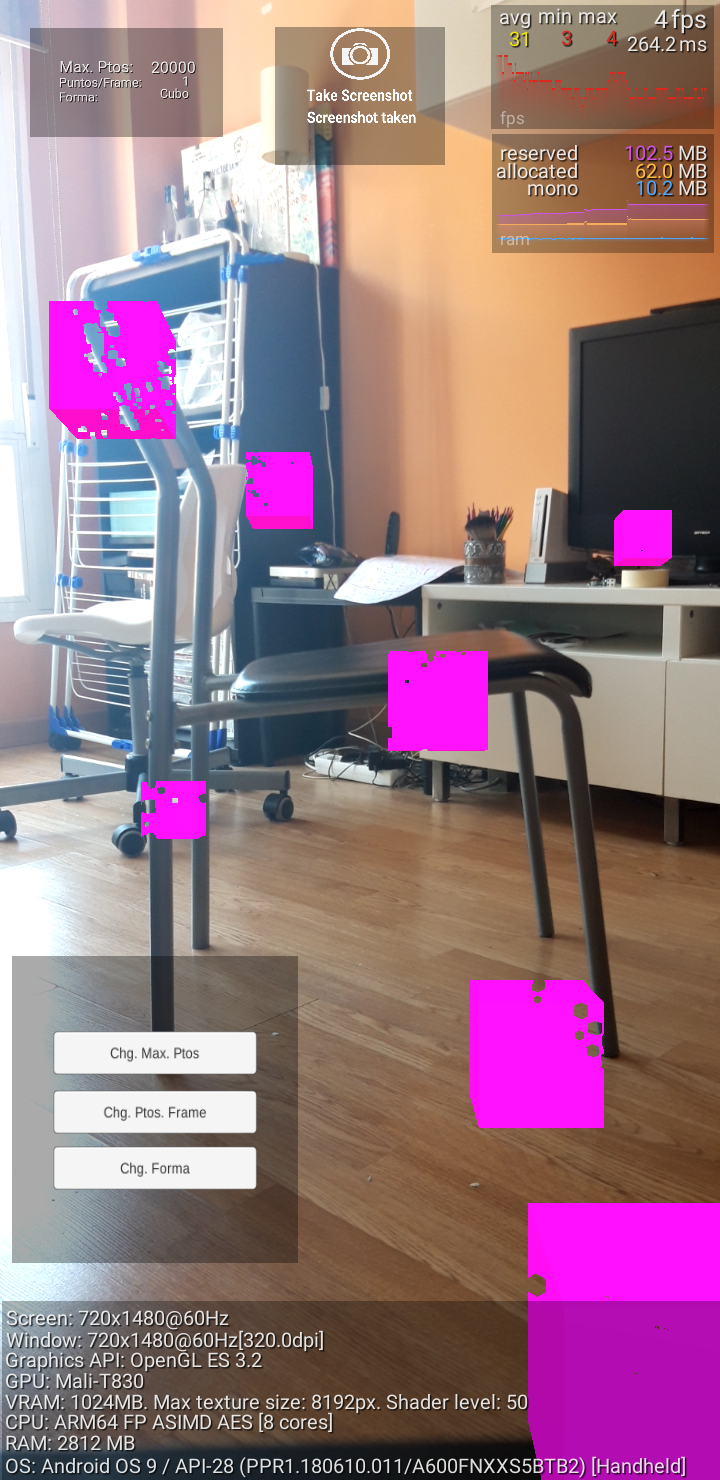
\includegraphics[scale=0.20]{Images/NubeDePuntos/AplicacionPruebas.jpg}
%    \caption[Aplicación para visualizar el rendimiento de la nube de puntos.]{Aplicación para visualizar el rendimiento de la nube de puntos \footnotemark.}
%    \label{fig:SFM}
%\end{figure} 